%%%%%%%%%%%%%%%%%%%%%%%%%%%%%%%%%%%%%%%%%%%%%%%%%%%%%%%%%%%%%%%%%%%%%%%%%%%%%%%%
%2345678901234567890123456789012345678901234567890123456789012345678901234567890
%        1         2         3         4         5         6         7         8

\documentclass[letterpaper, 10 pt, conference]{ieeeconf}  % Comment this line out if you need a4paper

%\documentclass[a4paper, 10pt, conference]{ieeeconf}      % Use this line for a4 paper

\IEEEoverridecommandlockouts                              % This command is only needed if 
                                                          % you want to use the \thanks command

\overrideIEEEmargins                                      % Needed to meet printer requirements.

\title{\LARGE \bf SwarmAvg: A Novel Approach to Fully Distributed Machine Learning}


\author{Josh Pattman$^{1}$% <-this % stops a space
}

\usepackage{graphicx}
\graphicspath{{./plots/}}

\usepackage{algpseudocode}
\usepackage{algorithm}
\usepackage{subcaption}
\usepackage{cite}

\begin{document}



\maketitle
\thispagestyle{empty}
\pagestyle{empty}


%%%%%%%%%%%%%%%%%%%%%%%%%%%%%%%%%%%%%%%%%%%%%%%%%%%%%%%%%%%%%%%%%%%%%%%%%%%%%%%%
\begin{abstract}

Federated learning is a technique that allows a machine learning model to be trained on data distributed across multiple data islands. This approach protects privacy by keeping the data decentralized, meaning that sensitive data does not need to ever be shared. Swarm learning is a similar technique that eliminates the need for a central server, ensuring that not only the data, but also the communication, is completely decentralized. Current Swarm Learning algorithms rely on blockchain to distribute the shared global model, however this may be a poor choice for certain scenarios closely associated with swarms. In this paper, a novel swarm learning technique called SwarmAvg is presented which operates without a blockchain. The algorithm is validated against federated learning in various scenarios, and also in some situations where federated learning cannot be applied. The benefits and drawbacks of operating Swarm Learning without a blockchain are also discussed, exemplifying some interesting reasons why one might choose to use SwarmAvg over other distributed machine learning techniques.

\end{abstract}


%%%%%%%%%%%%%%%%%%%%%%%%%%%%%%%%%%%%%%%%%%%%%%%%%%%%%%%%%%%%%%%%%%%%%%%%%%%%%%%%
\section{INTRODUCTION}

Machine learning is becoming an exceedingly vital tool for our society to progress. However, many modern machine learning algorithms require large volumes of diverse data to achieve optimal performance. In the ideal world, this data would be stored in a single location close to a very powerful computer for training. Unfortunately, real-world data is often distributed among multiple nodes that are unable to share the data with each other or a central location, due to privacy regulations such as GDPR \cite{gdpr}. Accessing a super computer for training is also a luxury that many cannot afford. The reduction in data volume available can negatively impact the post training performance \cite{data_volume}, and the use of a slower computer means that training may not be able to be performed as fast as needed.

\section{BACKGROUND}

Machine learning is an exceedingly vital tool in modern society. Nonetheless, as the issues which machine learning endeavours to resolve become more intricate, the possibility of utilising a single centralized intelligence diminishes. One possible remedy to this problem is the distribution of both data and computation amongst multiple nodes. Transitioning from centralized approaches to distributed approaches also offers numerous advantages. For example, it has been proven mathematically that the accuracy of a distributed system surpasses that of a centralized one \cite{swarmbetterthanone}. The following sections will provide an overview of some of the state-of-the-art approaches used to distribute machine learning.


\subsection{Federated Learning}
% Introduce federated learning
Federated Learning (FL) \cite{survey_on_fed_learning} is a technique in machine learning that aims to train a single model using all available data across nodes without requiring any data to be shared among them. \\

% Intro on how fed learning works and different types
There are a multitude of published FL frameworks \cite{fed_table_survey}, each with different merits and drawbacks for certain use cases. Federated Averaging (FedAvg) \cite{fed_learning} is a commonly used yet simple framework, which splits training into iterations where three steps take place:
\begin{enumerate}
	\item A copy of the current model is sent to each node from the central server.
	\item Each node performs some training with their copy of the model and their own private data.
	\item The trained models from each node are sent back to the server to aggregate into the new server model.
\end{enumerate}
The server model is improved over time, beyond what could be achieved by simply training on a the data stored on a single node. \\

% Specify why federated learning is better than conventional learning
As it does not require data to be shared between nodes, FL is naturally beneficial for privacy sensitive tasks compared to conventional machine learning where the data is aggregated in a central location \cite{fed_privacy}. Additionally, as FL performs training on multiple nodes in parallel, it can make better use of available training resources in situations where processing power is not only distributed among multiple nodes but also limited on each node, such as Internet of Things (IoT) \cite{fed_iot_2}.

% federate distributed
FL has been adapted into several variations which eliminate the need for a single central server. One such variant is Multi-Center Federated Learning \cite{multi_center_fed_learning}, which involves multiple central servers, each connected to different clusters of nodes. Another approach is to use leader election to select a node to function as the server \cite{fed_leaderelec}. This method can improve network resilience because, if the server fails, a new server is elected.

\subsection{Blockchain} \label{bg:bc}
% Breif intro of what a blockcahin is
Blockchain technology enables a network of nodes to record transactions on a shared ledger in a fully decentralized manner \cite{blockchain_review}. In a conventional blockchain, any participating node is permitted to add a transaction to the ledger, but once a transaction is executed, it becomes immutable and irreversible. Although blockchains are primarily associated with cryptocurrency and financial transactions, any type of data, including neural network weights, can be recorded as a transaction. \\

% Disadvantages of using blockchain
When a blockchain is scaled up, it may encounter performance issues. For instance, the Bitcoin network typically processes only 7 transactions per second on average \cite{blockchain_scale}. High confirmation delay and performance inefficiency are two primary issues related to this paper when scaling up a blockchain \cite{blockchain_scale}. These issues could prove catastrophic in a system like a swarm of robots, where it is crucial to always have the latest data and optimize limited processing power.

\subsection{Swarm Learning}
% Introduce swarm learning
Swarm Learning (SL) is a subcategory of FL which operates in a completely distributed and decentralised manner. SL enables the collaboration of nodes to learn a shared global model, however in contrast to FL, a central server is never used. SL also does not use leader election, so all nodes on the network are given the same importance. \\

In SL, the model on which new training is performed is known as the global model. However, unlike FL where the global model is stored in a central location, the global model in SL does not materially exist, but is instead a concept which is agreed upon by the nodes in the network. An illustration of the different algorithms is shown in Figure \ref{fig_learning}. \\

\begin{figure}[h]
	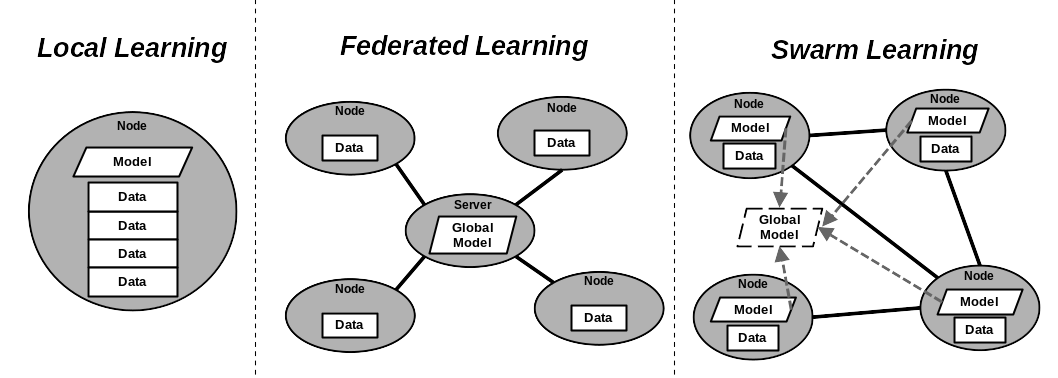
\includegraphics[width=\linewidth]{fedvsswarm}
	\caption{Diagram of different learning algorithms. Each \emph{Node} indicates a single training machine, and each line denotes a connection between two machines, along which the model can be shared. In the swarm learning diagram, the dashed lines show that each local model is an approximation of the global model.} \label{fig_learning}
\end{figure}

One SL algorithm, referred to by this paper as SwarmBC, uses a blockchain to store the global model \cite{swarm_learning}. In this version of SL, training is performed by repeating the following steps:
\begin{enumerate}
	\item A node obtains a copy of the global model from the blockchain.
	\item The node performs some training with their copy of the model and their own private data.
	\item The updated model is merged with the latest blockchain model and sent back to the blockchain for other nodes to use.
\end{enumerate}

% Specify why swarm learning is better than conventional learning or federated learning
SL exhibits many of the same benefits of FL over conventional learning, but it also improves upon FL in some aspects. As is often the case when comparing decentralised algorithms to their centralised counterparts \cite{swarm_resil}, the absence of a central server theoretically makes SL more resilient and robust to failures than centralized FL approaches such as FedAvg. The absence of a central server in SL not only means that the system does not entirely rely on a single node, but also that it is less sensitive to disruptions in connections between nodes. In FL, if a connection between two nodes ceases to exist, the node can no longer participate in learning without some form of tunnelling. In contrast, in SL, even if a connection between two nodes is lost, the two connected nodes are still likely to be connected to other operational nodes, enabling the system to continue functioning normally. \\

The utilisation of FL with leader election effectively addresses the challenge of ensuring system robustness, as it enables any node to serve as a replacement for the server in the event of network disconnection. Nevertheless, it is important to note that a swarm of nodes is not often completely interconnected, and the connections between the nodes are often subject to changes. This dynamic and sparse network topology can present significant complexities when it comes to leader election, leading to an increase in overhead \cite{leaderelection}. The lack of a leader election process in SL makes it a more viable option in such situations. \\

Finally, a swarm of nodes can offer greater scalability compared to its centralized counterpart, particularly if agents are restricted to communicating with only their nearby neighbours \cite{swarmscalable}. This is primarily because in such cases, there is no need for all communications to travel to a single node or server that may not be able to handle the significant volume of traffic. In a swarm, where nodes are limited to a certain number of close neighbours, the size of the swarm becomes less significant, since a single node would not experience a difference between a small or large swarm, as it would have the same number of neighbours. Consequently, SL is typically more scalable than FL.


\section{Algorithm Design} \label{des}
\subsection{Design Overview}
In SL, a node is an agent responsible for facilitating the improvement of the global model. The global model is an abstract concept representing the consensus of all nodes in the network. In the proposed version of SL, referred to as SwarmAvg, each node maintains its own model, known as the local model, which is an approximation of the global model. However, in SwarmAvg, the consensus algorithm used is repeated averaging, not blockchain like in SwarmBC. This means that at the start of each training step, every node may start with a slightly different model. As training progresses and performance begins to plateau, each node's local model should not only converge towards a minima with respect to loss, but also towards each other. \\

Each node in the network possesses a confidential dataset that is not disclosed to any other nodes. In order to train the global model, nodes fit their own local model of their local dataset. In order to maintain consistency between local and global models, a combination procedure is conducted following each round of local training, which involves the integration of neighbouring nodes models into the local model. \\

SwarmAvg works by repeating the training step until training is complete. The actions in each training step for SwarmAvg are as follows:
\begin{enumerate}
	\item Fit local model to local dataset.
	\item Send local model to all neighbours.
	\item Combine neighbouring models into local model, using one of the methods presented in Section \ref{mcm}.
\end{enumerate}

Additionally, each node retains a local cache of the most recent models of its neighbouring nodes. This cache is updated each time a neighbouring node transmits its model to the node in question, instead of being updated on-demand during the combination step. The reasoning behind this decision is explained further in Section \ref{reasonforcache}.

\subsection{The Algorithm}
The training step, found at Algorithm \ref{updatealgo}, is the section of the algorithm which runs continuously during the time which a node is running. It takes care of training and synchronising the local model. The provided code represents what happens in a single training step, meaning that it should be run in a loop that terminates once a stop condition, such as target accuracy, has been reached.

\begin{algorithm}[H]
	\caption{A Single Training Step - should be called repeatedly in a loop} \label{updatealgo}
	\begin{algorithmic}[1]
		\State \Call{Train}{localModel, localData}
		\ForAll{$n \in neighbors$}
		\State \Call{SendTo}{$(localModel, localTrainingCounter)$, $n$}
		\EndFor
		
		\For{$x \in range(maxSyncWaits)$}
		\State $neighborModels \gets \emptyset$
		\ForAll{$n \in neighbors$}
		\State $model, traningCounter \gets$ \Call{CacheLookup}{$n$}
		\If{$trainingCounter + \beta \ge localTrainingCounter$}
		\State \Call{Append}{$neighborModels$, $model$}
		\EndIf
		\EndFor
		\If{$length_{neighborModels} \ge \gamma$}
		\If{$syncronisationMethod = "AVG"$}
		\State $localModel \gets \mu(localModel \cup neighborModels)$
		\ElsIf{$syncronisationMethod = "ASR"$}
		\State $localModel \gets (1 - \alpha) * localModel + \alpha * \mu(neighborModels)$
		\EndIf
		\Else
		\State continue
		\EndIf
		\State \Call{Sleep}{syncWaitTime}
		\EndFor
	\end{algorithmic}
\end{algorithm}

The model received event, which can be found at Algorithm \ref{cachealgo}, is run on the local node every time a remote node sends the local node a model update. This event takes care of updating the local model cache, to ensure the local node has the most up-to-date information. The model update sent from the remote node should contain the model and training counter of the remote node.

\begin{algorithm}[H]
	\caption{Model Received Event - called when a model update is received from a remote node} \label{cachealgo}
	\textbf{Input}: $neighbour$, $nModel$, $nTrainingCounter$
	\newline
	\begin{algorithmic}[1]
		\If{\Call{InCache}{$neighbour$}}
		\State $\_, nTraningCounterOld \gets$ \Call{CacheLookup}{$n$}
		\If{$nTrainingCounter > nTraningCounterOld$}
		\State \Call{SetCache}{$neighbour$, $(nModel, nTrainingCounter)$}
		\EndIf
		\Else
		\State \Call{SetCache}{$neighbour$, $(nModel, nTrainingCounter)$}
		\EndIf
	\end{algorithmic}
\end{algorithm}

\subsection{Blockchain-less Algorithm}
Whereas SwarmBC employs a blockchain as the mechanism for distributing the global model, SwarmAvg utilises a variation of averaging with its neighbours and does not use a blockchain. This decision was made due to the long transaction confirmation time of large blockchains, which could adversely affect training as nodes continuously upload their latest networks to the network. If this process were to take an excessive amount of time, each node would be training on an outdated model. \\

Furthermore, the inefficiency of blockchains with respect to performance is another reason for not using them in SwarmAvg. SwarmAvg is designed for deployment in large swarms, with each agent possibly having low processing power. If a blockchain were utilised, some of the processing power that could be devoted to training would instead be utilised for validating transactions. In scenarios where processing power is limited, it would be practical to avoid the use of blockchains.

\subsection{The Training Counter}
A vital aspect of SwarmAvg, specifically the combination step, involves evaluating the performance of a nodes local model. The conventional approach would involve testing each model using an independent test set. However, due to the inability to exchange test sets among nodes, this approach is not feasible as it would result in non-comparable scores for each model. In order to circumvent this problem, this paper presents a heuristic metric referred to as the "training counter," which serves as an approximation of the level of training for a network by estimating the number of training steps performed on a given model. \\

The training counter can be changed in one of two manners. Firstly, the counter is incremented by 1 when the local model is trained on the local dataset, indicating that an additional step of training has been performed. Following the combination step, the training counter is also updated to reflect the how the models were combined. For instance, if the neighbouring models were simply averaged, the training counter would be updated to represent the average of all neighbouring nodes' training counters.

\subsection{Combining Neighbouring Models} \label{mcm}
The combination step is a crucial component of SwarmAvg. During this step, a node merges its local model with those of its neighbours, producing an updated estimate of the global model.

In the below equations, $\mu(x)$ denotes the function $mean(x)$. All models are assumed to be flattened into 1-dimensional arrays of parameters.

The method of combination used by this paper is called Averaging with Synchronisation Rate (ASR). This involves computing the average model of all neighbours, then calculating the weighted mean between that model and the local model.
\[ localModel \gets (1 - \alpha) * localModel + \alpha * \mu(neighborModels) \]
The synchronisation rate, denoted as $\alpha$, indicates the degree to which each node adjusts its local model to align with the global model. If $\alpha$ is set too low, each node's model in the network will diverge, resulting in each node becoming trapped at a local minima, an effect referred to as divergent training. On the other hand, if $\alpha$ is too high, the progress achieved by the local node will be discarded at each averaging step, which can result in slower learning. \\

This method is beneficial over simply averaging all known models, as it provides some resistance to variation in the number of neighbours of a node. When using simple averaging, the amount of change made by the local node that persists into the next training step is inversely proportionate to the number of neighbours which were combined. However, when using averaging, the amount of change made that persists will be constant, no matter how many neighbours that are present. This may increase the stability of training, especially if the situation which SwarmAvg is deployed involves a dynamic set of neighbours.

\subsubsection{Training Counter Filtering}
A potential modification to the previously mentioned combination algorithm involves filtering based on the training counter. Specifically, a node may only include its neighbour models if they meet the following statement:
\[neighborTrainingCounter + \beta \ge localTrainingCounter \]
The training offset $\beta$ is the amount the training counter of a neighbour can be behind the local training counter before it is ignored. \\

A compelling reason to allow training counter filtering is the increased fault tolerance. Consider the situation where node \emph{A} has received many model updates from many nodes, one of which being node \emph{B}. However, node \emph{B} goes offline and no longer is sending model updates. Without training counter filtering, node \emph{A} will continue to combine the outdated node \emph{B} model with it's own for as long as it is training. However, if training counter filtering is enabled, after a number of training steps the outdated model \emph{B} updates will be ignored. \\

An issue with training counter filtering pertains to the presence of runaway nodes. These nodes possess a substantially higher training counter compared to all other nodes in the network, meaning that when filtering is applied, they are left with no neighbours to utilise in the combination step. Consequently, a runaway node may start to overfit on its own training data, as this is the only data it is exposed to, thereby leading to decreased local performance, as well as potential performance reductions in the rest of the network. To address this problem in SwarmAvg, each node must wait until it has obtained at least $\gamma$ viable neighbours prior to performing the combination step. Although this measure prevents individual nodes from becoming runaway nodes, groups of size $\gamma$ still have the potential to become runaway as a unit. Nevertheless, if $\gamma$ is roughly equivalent to the number of neighbours and all neighbours train at a comparable rate, the issue is minimised.

\section{Strategy for Gathering of Results}
The experiments were conducted through the simulation of a group of nodes on a single computer. The accuracy of each node was evaluated on an unseen test set and subsequently recorded in a file after each training step. All nodes shared the same test set. Below are the specific details of the running of each experiment:
\begin{description}
	\item [Chosen Metric: Accuracy:] The metric chosen for the following experiments was accuracy, due to its comprehensible nature. Despite the fact that an unbalanced dataset presents one of the significant drawbacks of using accuracy, this concern is irrelevant in the case of the chosen dataset, MNIST Fashion (MNIST-F), since it is a balanced dataset, meaning it has the same number of samples in each class. The accuracy of each node is computed after each training step using the test subset of MNIST-F, and none of the nodes are ever provided access to the test set for training.
	
	\item [Number of Simulated Nodes:] The experiments were conducted using 10 nodes, with the exception of the server in cases where FedAvg was employed. The decision of how many nodes to simulate was based on the highest node count attainable without causing inconsistencies and crashes due to resource depletion of the training machine.
	
	\item [Repeated Testing for Noise Reduction:] The training process for each experiment was conducted five times, and the resulting accuracies of every node were recorded. To mitigate the impact of training noise on the performance graphs, the accuracy value for each time step was calculated as the median accuracy across all nodes and runs at that time step. As there were 10 nodes, this resulted in the graphs representing median of 50 nodes.
	
	\item [Configuring the Algorithm:] In each of the following experiments, the algorithm was configured using a specific set of parameters $\alpha \beta \gamma$. These parameters were obtained heuristically by making an initial guess, testing, and then fine-tuning them until a satisfactory outcome was reached. However, it is important to note that an exhaustive investigation into the optimal parameter configuration for a particular type of problem is not within this papers scope, meaning that it is plausible that swarm learning could yield better results with more precisely tuned parameters.
	
	\item [Data Provided to Each Node:] The experiments evaluate the algorithm's performance using three levels of data volume per node. These levels are considerably smaller than the full MNIST-F dataset not only to increase problem difficulty, but also as the algorithm is intended for scenarios where each nodes access to data is restricted. To create a subsection of data for each node, a random sampling with replacement method was used to select the desired number of datapoints. During the initial training phase, each node performs a single sampling of its dataset, after which that nodes data subset remains constant. The three levels of data volume can be seen in Table \ref{epsparams}.
	
	\item [Training Steps and Epochs:] Due to the limited size of the dataset, a single node executes more than one epoch of training in each training step. The number of epochs carried out by a node per training step will be referred to as Epochs per Step (EPS). Empirical testing has indicated that both SL and FL exhibit improved performance with higher EPS, at times surpassing the gains from increasing the number of training steps. Moreover, the utilisation of higher EPS was favoured due to its reduced training time, compared to increasing the number of training steps. The three levels of data volume with their respective EPS are shown in table \ref{epsparams}.
	
\end{description}

\begin{table}[H]
	\centering
	\begin{tabular}{l|l}
		Dataset Size & EPS \\ \hline \hline
		1000   & 5  \\ \hline
		100   & 10  \\ \hline
		25  & 20 
	\end{tabular}
	\caption{The different levels of dataset size and EPS that were tested} \label{epsparams}
\end{table}

\section{Results}
\subsection{Sparsely Connected Network of Nodes}
In reality, it is uncommon for each node to be linked with every other node. To simulate a more realistic scenario, a technique was employed to generate a network of nodes with a specific number of connections. When density is set to 0, the network is minimally linked, meaning that each node has at least one indirect path to every other node, but the minimal number of connections required to accomplish this exist. When density is set to 1, all nodes are connected to one another in a dense fashion. Since this measure may not provide a straightforward indicator of network density, two additional metrics will be provided:  Mean Minimum Hops (MMH) and Mean Connections per Node (MCPN). MMH denotes the mean minimum number of transitions required to get from one node to another in the network. MCPN denotes the average number of connections a given node possess, for a network of 10 nodes. \\

In order to conduct thorough testing on a variety of potential deployment scenarios, several different densities were tested for each count of data. The densities that were tested, along with their corresponding MMH and MCPN, are presented in Table \ref{sparsedensities}.

\begin{table}[H]
	\centering
	\begin{tabular}{l|l|l}
		Density & MMH & MCPN \\ \hline
		1 & 1.0 & 9.0 \\
		0.75    & 1.2 & 7.2  \\
		0.5    & 1.4 & 5.4  \\
		0.25    & 1.7 & 3.6  \\
		0    & 3.0 & 1.8  \\
	\end{tabular}
	\caption{The statistics for different density levels} \label{sparsedensities}
\end{table}

In order to assist the reader with visualizing the various density levels, some sample networks that were generated for each density can be found in Figure \ref{densefig}.

\begin{figure}[H]
	\centering
	\begin{subfigure}[b]{0.3\textwidth}
		\centering
		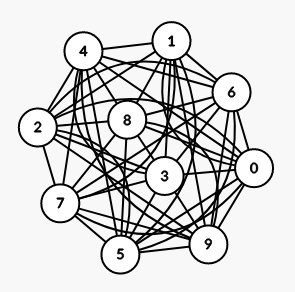
\includegraphics[width=\textwidth]{sparsegraph100}
		\caption{$density=1.0$}
	\end{subfigure}
	\begin{subfigure}[b]{0.3\textwidth}
		\centering
		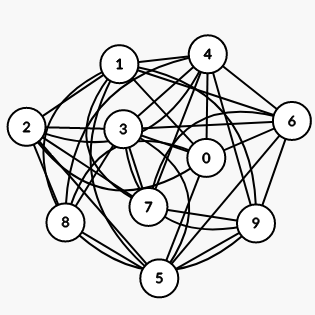
\includegraphics[width=\textwidth]{sparsegraph75}
		\caption{$density=0.75$}
	\end{subfigure}
	\begin{subfigure}[b]{0.3\textwidth}
		\centering
		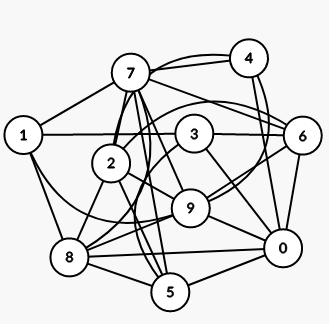
\includegraphics[width=\textwidth]{sparsegraph50}
		\caption{$density=0.5$}
	\end{subfigure}
	\begin{subfigure}[b]{0.3\textwidth}
		\centering
		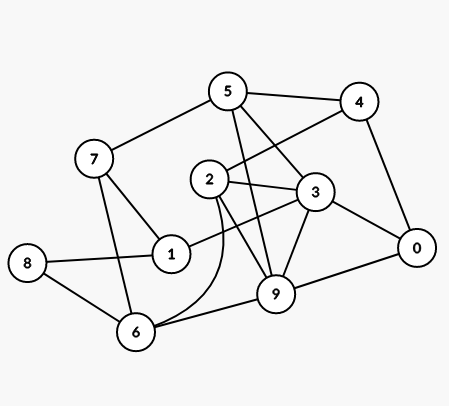
\includegraphics[width=\textwidth]{sparsegraph25}
		\caption{$density=0.25$}
	\end{subfigure}
	\begin{subfigure}[b]{0.3\textwidth}
		\centering
		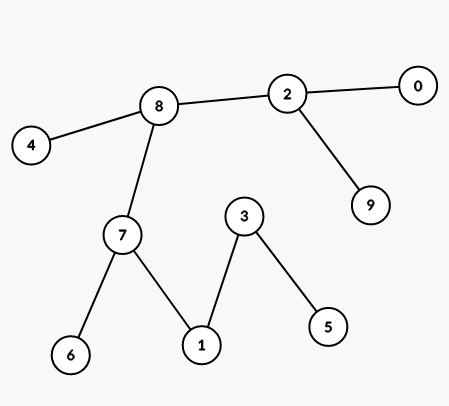
\includegraphics[width=\textwidth]{sparsegraph0}
		\caption{$density=0.0$}
	\end{subfigure}
	\caption{Example networks of nodes generated for each density level, visualised using the tool at \emph{https://csacademy.com/app/graph\_editor}. Each time a simulation is started, a new random network is generated for that simulation. \label{densefig}}
	{}\end{figure}


This section does not include any testing of FedAvg. In scenarios where not every node is directly connected to the server node, FedAvg has two potential options: ignore all nodes which are not directly connected, or attempt to relay the model updates through connected nodes. As mentioned in Section \ref{relay}, relaying may not always be the optimal solution. Ignoring nodes is also not a good option, as data is wasted. Therefore, in this test, the decision was made to solely evaluate SwarmAvg.

Below are results obtained from testing. The density of each line on the graph is indicated by the colour, with a green hue representing higher density and a red hue indicating lower density. For all tested densities, the value of $\gamma$ was set to $round_{down}(MCPN) - 1$, which ensures that each node can progress only after waiting for all but one of its neighbours. Notably, failure to reduce $\gamma$ for less dense networks would cause several nodes to wait for a number of neighbours that cannot be achieved. Due to the random nature of the graph generation, there will still be some nodes who have less than $\gamma$ neighbours, but this should be rare and the loop to wait for $\gamma$ neighbours will terminate after a certain number of tries anyway, ensuring that training can progress.

\begin{figure}[H] 
	\center{\textbf{Accuracy by Training Step for 1000 Samples, with Varying Density}} \\
	\begin{subfigure}{0.49\textwidth}
		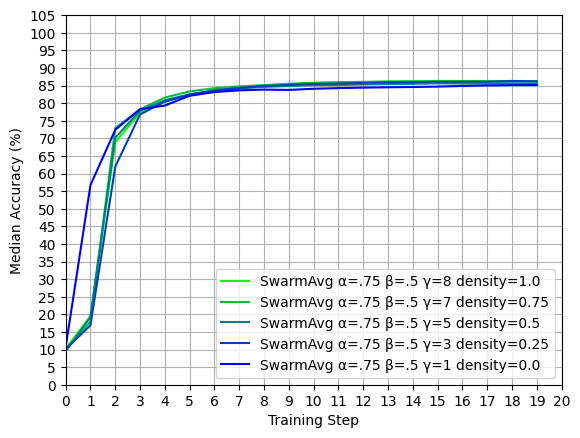
\includegraphics[width=\textwidth]{aeg_sparse_1000}
		\caption{Full Graph}
	\end{subfigure}
	\begin{subfigure}{0.49\textwidth}
		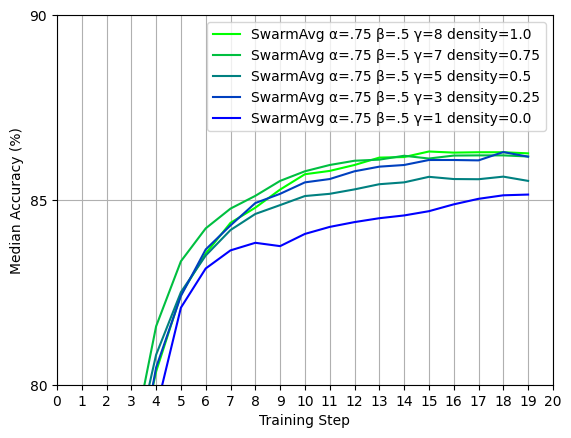
\includegraphics[width=\textwidth]{aeg_sparse_1000_z}
		\caption{Zoomed Graph}
	\end{subfigure}
	\caption{Median accuracy by training step across 5 repeats. Each node has 1000 random data samples from MNIST-F. Quartiles are not shown.}
	\label{aeg4}
\end{figure}

An observation that can be made of Figure \ref{aeg4} is that the different network densities perform very similarly. The final accuracy for all of the tests fell within a 2 percent range,  with the higher densities occupying the higher end. \\

One interesting feature of the Figure \ref{aeg4} is that the lowest density demonstrates faster convergence initially that the other densities. The author hypothesises that this may be due to groups of nodes forming local sub-networks which converge on their own sub-sets of data faster, but more slowly combine into the network as a whole as training progresses.

\begin{figure}[H] 
	\center{\textbf{Accuracy by Training Step for 100 Samples, with Varying Density}} \\
	\begin{subfigure}{0.49\textwidth}
		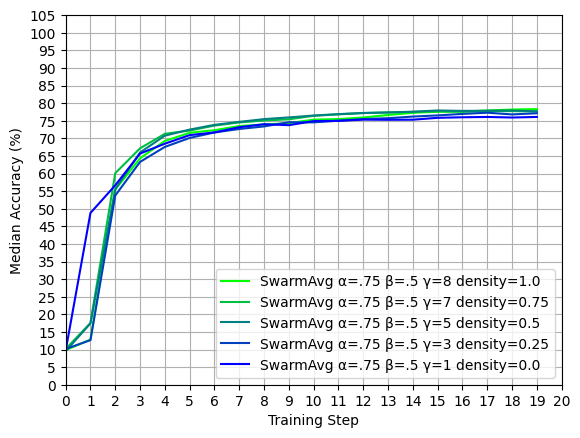
\includegraphics[width=\textwidth]{aeg_sparse_100}
		\caption{Full Graph}
	\end{subfigure}
	\begin{subfigure}{0.49\textwidth}
		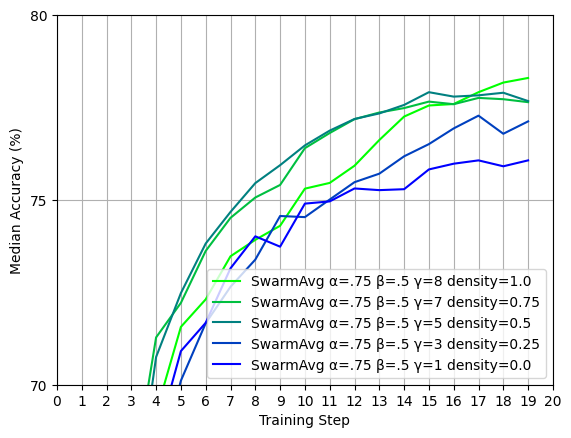
\includegraphics[width=\textwidth]{aeg_sparse_100_z}
		\caption{Zoomed Graph}
	\end{subfigure}
	\caption{Median accuracy by training step across 5 repeats. Each node has 100 random data samples from MNIST-F. Quartiles are not shown.}
	\label{aeg5}
\end{figure}

In Figure \ref{aeg5}, there is a greater spread of final accuracies, about 2.5 percent, than is shown in Figure \ref{aeg4}. The more noticeable feature of Figure \ref{aeg5} is that the final accuracies of all densities are approximately 8 percent lower than their counterparts with more data available in figure \ref{aeg4}.

\begin{figure}[H] 
	\center{\textbf{Accuracy by Training Step for 25 Samples, with Varying Density}} \\
	\begin{subfigure}{0.49\textwidth}
		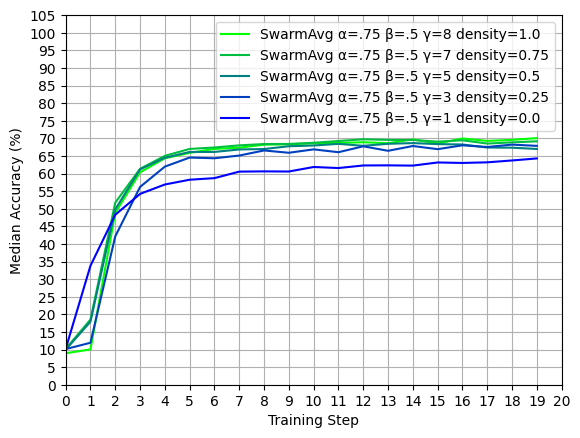
\includegraphics[width=\textwidth]{aeg_sparse_25}
		\caption{Full Graph}
	\end{subfigure}
	\begin{subfigure}{0.49\textwidth}
		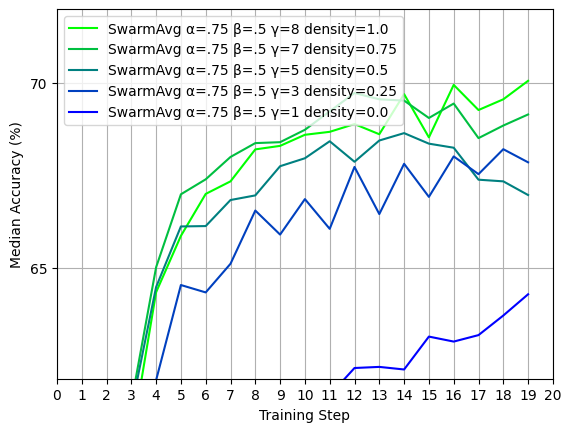
\includegraphics[width=\textwidth]{aeg_sparse_25_z}
		\caption{Zoomed Graph}
	\end{subfigure}
	\caption{Median accuracy by training step across 5 repeats. Each node has 25 random data samples from MNIST-F. Quartiles are not shown.}
	\label{aeg6}
\end{figure}

With 25 data samples, the tests depicted in Figure \ref{aeg6} show a much higher variation in final accuracies than the previous two figures. There is also a much higher degree of noise in this figure than any other, suggesting that training may be much less stable with this small number of data samples to train on.

It should also be noted that the lowest density is still exhibiting the behaviour of outperforming the other densities in the initial steps, however it appears that this effect has become slightly less prominent. \\


Generally, altering the network density of nodes has a small impact on the training of the nodes within the network. Decreasing the density of nodes typically leads to a lower final accuracy. This effect becomes more noticeable as the data volume provided to each node decreases, as demonstrated by the increased variability in training displayed in Figure \ref{aeg6} in comparison to Figures \ref{aeg4} and \ref{aeg5}. \\

The networks possessing a density of 0 attain their optima at a faster rate than those with higher densities. Figure \ref{aeg6} illustrates that the lower densities reach convergence marginally quicker than higher densities, yet are surpassed by the latter towards the end of training.

\subsection{Scenario 4: Sparsely Connected Network with Class Restrictions}
Decentralized machine learning algorithms, such as SwarmAvg, commonly involve a scenario where each node possesses a dataset whose distribution does not align with the overall data distribution across all nodes. In order to simulate such a scenario, a situation was created where each node was given access a unique set of three out of ten classes of MNIST-F. The performance of SwarmAvg was tested for each density level.

Below are the results.
\begin{figure}[H] 
	\center{\textbf{Accuracy by Training Step for 1000, 100 and 25 Samples, with 3 Classes and Varying Density}} \\
	\begin{subfigure}{0.49\textwidth}
		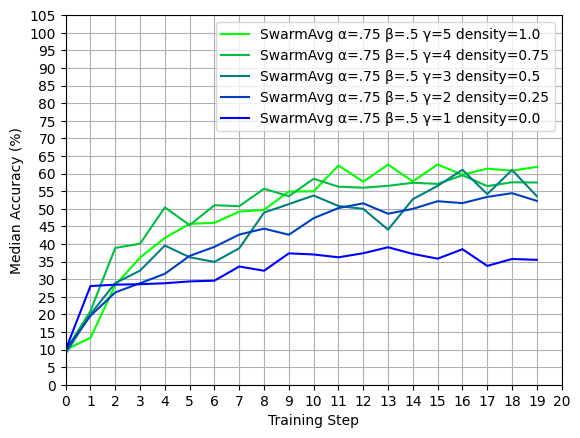
\includegraphics[width=\textwidth]{aeg_sparse_unev_1000}
		\caption{Samples=1000}
	\end{subfigure}
	\begin{subfigure}{0.49\textwidth}
		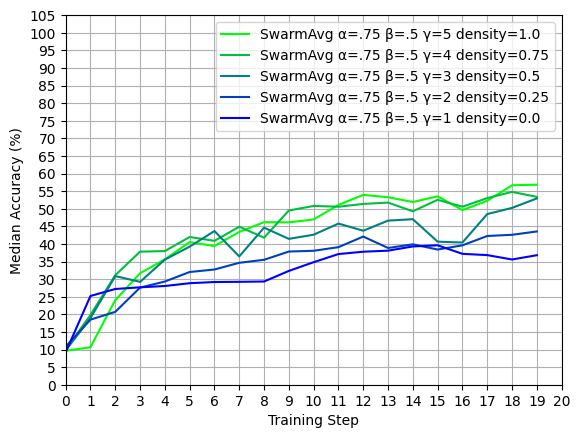
\includegraphics[width=\textwidth]{aeg_sparse_unev_100}
		\caption{Samples=100}
	\end{subfigure}
	\begin{subfigure}{0.49\textwidth}
		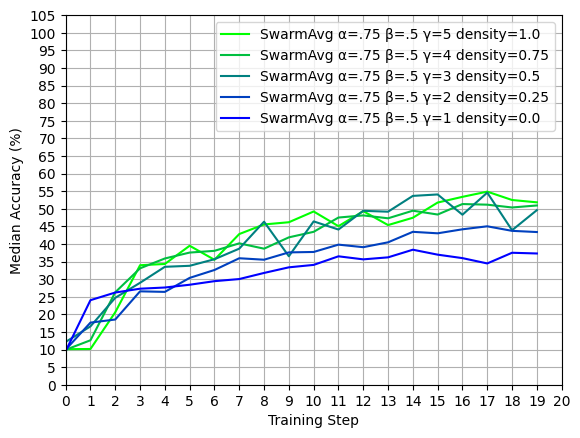
\includegraphics[width=\textwidth]{aeg_sparse_unev_25}
		\caption{Samples=25}
	\end{subfigure}
	\caption{Median accuracy by training step across 5 repeats. Quartiles are not shown. Each node has access to a unique set of 3 classes out of 10.}
	\label{aeg9}
\end{figure}


In all three tests, it is clear that a higher density is highly correlated with higher performance in this scenario. It is also noteworthy that with a network density of 0, no matter which volume of data was presented, the accuracy curve was very similar. However, as the density of the network increased, so did the degree at which it was effected by the reduction in data. This scenario also presented graphs with a high degree of noise when compared to other scenarios, despite representing the median of 5 training runs. However, the level of noise is somewhat consistent on all three tests with different data volumes.

\section{Comparison of SwarmAvg to Other Methods}
Although SwarmAvg has demonstrated promising results, it remains important to conduct a comparative analysis against established methods. This will enable individuals seeking to incorporate distributed machine learning into their future projects to make an informed decision whether SwarmAvg is the algorithm that they should use.

\subsection{Comparison of SwarmAvg to FedAvg}
SwarmAvg has the significant benefit of being more fault tolerant than FedAvg. This is because FedAvg has a central server, which means that the whole network would stop functioning if the central server is stopped. Not only this, but if a node drops its connection to the server, that node is effectively ignored from training, which has a negative effect on performance. \\

However, SwarmAvg has some significant drawbacks. For example, SwarmAvg has been shown to be slower to converge than FedAvg. Not only this, but SwarmAvg can create a significantly higher amount of network traffic than FedAvg or FL in general. This effect is maximised when every node is connected to every other node, meaning that the number of connections scale by $O(n^2)$, where $n$ is the number of nodes. FL will always both number of connections and network traffic scale with $O(n)$, as every node only needs a single connection to the server. However, it is worth noting that SwarmAvg will consume less network traffic in less dense networks of nodes. \\

An important advantage of SwarmAvg over FedAvg is that former can be used in sparsely connected networks without any modification. This means that it is possible for it to SwarmAvg to run even when most nodes in the network are not connected to most other nodes, which may be a more realistic scenario for certain low powered networks of devices such as IoT networks or robotic swarms. For this reason, SwarmAvg may be a better choice than FedAvg for these situations.

\subsection{Comparison of SwarmAvg to SwarmBC}
Despite the fact that this paper did not perform tests on SwarmBC, it is still possible to theoretically compare both SwarmAvg and SwarmBC, based on a comprehensive understanding of the inner workings of each. \\

One of the primary drawbacks of utilising SwarmAvg as opposed to SwarmBC is the potential occurrence of divergent training during SwarmAvg training. The detrimental effect of divergent training may persist throughout the entire training process, leading to significantly worse performance than anticipated. Several factors can lead to divergent training, with low settings for $\alpha$ and $\gamma$, coupled with a sparsely-connected network, being highly correlated with its occurrence during testing. SwarmBC does not suffer from this issue, as the blockchain ensures that all nodes agree on the same model. However, during testing, divergent training was a rare phenomenon, and its remedy was a simple parameter tuning process upon detection. \\

One drawback of utilising the SwarmAvg algorithm, as opposed to SwarmBC, is the absence of security features. The utilisation of blockchain technology enables the straightforward authentication of nodes utilising different algorithms that are frequently well-documented and integrated into the blockchain framework. On the other hand, SwarmAvg lacks any built-in authentication mechanism. As a result, to employ it securely, a separate authentication system would need to be implemented to prevent malicious parties from interfering with training. \\

SwarmAvg surpasses SwarmBC in terms of computational efficiency as nodes are not mandated to verify transactions with a blockchain, which involves a comparatively substantial overhead as opposed to simply averaging the models of a nodes neighbours. Consequently, SwarmBC necessitates higher processing power to operate for the same amount of training steps. This overhead could impede the speed of training on a resource-limited system, such as a swarm of drones, as a considerable amount of time is consumed in validating transactions, rather than performing training. Thus, SwarmAvg may be a more fitting choice than SwarmBC for swarms where processing power is a concern.

\addtolength{\textheight}{-12cm}   % This command serves to balance the column lengths
                                  % on the last page of the document manually. It shortens
                                  % the textheight of the last page by a suitable amount.
                                  % This command does not take effect until the next page
                                  % so it should come on the page before the last. Make
                                  % sure that you do not shorten the textheight too much.

%%%%%%%%%%%%%%%%%%%%%%%%%%%%%%%%%%%%%%%%%%%%%%%%%%%%%%%%%%%%%%%%%%%%%%%%%%%%%%%%



%%%%%%%%%%%%%%%%%%%%%%%%%%%%%%%%%%%%%%%%%%%%%%%%%%%%%%%%%%%%%%%%%%%%%%%%%%%%%%%%



%%%%%%%%%%%%%%%%%%%%%%%%%%%%%%%%%%%%%%%%%%%%%%%%%%%%%%%%%%%%%%%%%%%%%%%%%%%%%%%%
\section*{APPENDIX}

Appendixes should appear before the acknowledgment.

\section*{ACKNOWLEDGMENT}

I would like to thank my supervisor, Dr Mohammad Soorati, for supporting and inspiring me throughout the project, and really helping me to learn a lot more about the topic of this report.\\

I would also like to thank my secondary supervisor, Dr Jo Grundy, for always being fast to respond to any questions I have had, and always being willing to help out.\\

Finally, I would like to thank my peers James Harcourt, Daniel Say, Jack Darlison, and Siobhan Tinsley for having engaging discussions with me about the direction of my project, and always providing helpful critical feedback.



%%%%%%%%%%%%%%%%%%%%%%%%%%%%%%%%%%%%%%%%%%%%%%%%%%%%%%%%%%%%%%%%%%%%%%%%%%%%%%%%

References are important to the reader; therefore, each citation must be complete and correct. If at all possible, references should be commonly available publications.



\bibliographystyle{ieeetr}
\bibliography{final}{}


\end{document}
